\documentclass[11pt]{article}
\usepackage[russian]{babel}
\usepackage{fullpage}
\usepackage[T1]{fontenc}
\usepackage[utf8]{inputenc}
\usepackage{graphicx}
\usepackage{caption}
\usepackage{subcaption}
\usepackage{hyperref}
\usepackage{pdfpages}
\usepackage{gnuplot-lua-tikz}
%\usepackage{amsmath,amssymb}
\title{CGMIPT 2013 - Postscript Task}
\author{Денис Анисимов}

\pdfcompresslevel0

\begin{document}
\maketitle
\section*{Реализация}
В качестве тестовой таблицы была выбрана USAF-1951. Таблица представляет собой набор групп из 6ти элементов. Каждый элемент состоит из 3х вертикальных и трёх горизонтальных полос. Относительные размеры линий элемента показаны на рисунке \ref{fig:elem}. Ширина линии($0.5x$) в микрометрах для каждой группы показана в таблице \ref{tab:width}. 

Тестовая таблица(ps2pdf рендер для postscript кода) приведёна в конце данного документа.
\begin{figure}[!h]
  \begin{center}
  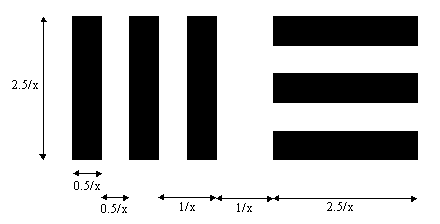
\includegraphics[scale=0.5]{USAFTestElementSpec.png}  
  \caption[Элемент таблицы]{Элемент таблицы\protect\footnotemark}
  \label{fig:elem}
  \end{center}
\end{figure}
\footnotetext{Источник:\url{http://www.efg2.com/Lab/ImageProcessing/TestTargets/}}

\begin{table}[!h]
\begin{center}
\begin{tabular}{lllllll}
& \multicolumn{6}{c}{Группа}\\
Элемент & -2 & -1 & 0  & 1 & 2 & 3 
\\
1 & 2000.00& 1000.00& 500.00 & 250.00 & 125.00 & 62.50
\\
2 & 1785.71& 891.27 & 446.43 & 223.21 & 111.36 & 55.68
\\
3 & 1587.30& 793.65 & 396.83 & 198.41 & 99.21 & 49.50
\\
4 & 1416.43& 707.21 & 354.61 & 176.68 & 88.34 & 44.25
\\
5 & 1259.45& 630.52 & 314.47 & 157.73 & 78.74 & 39.37
\\
6 & 1123.60& 561.17 & 280.90 & 140.45 & 70.13 & 34.97
\end{tabular}
\caption{Ширина одной линии в микрометрах}
\label{tab:width}
\end{center}
\end{table}

\section*{Растеризация}
Размер файла для различных значений разрешающей способности и различных форматов приведён в таблице \ref{tab:sizes} и на рисунке \ref{fig:sizes}. Для двух форматов также получены изображения со сглаживанием с размером блока 4x4. Для получения растрового изображения использовалась программа \texttt{ghostscript} с соответствующими опциями устройства вывода и сглаживания.

\begin{table}[h]
\begin{center}
	\begin{tabular}{llllllll}

	&\multicolumn{7}{c}{DPI} \\
	Формат & 36 & 72 & 144 & 200 & 300 & 600 & 1200\\
	pngmono  &  3692 & 5403 & 9385 & 12988 & 21140 & 55821 & 165173 \\
	pngalhpa  &  9509 & 18227 & 37684 & 55017 & 90939 & 247469 & 776750 \\
	png256 & 5308 & 8511 & 16504 & 24226 & 42132 & 108737  & 301216 \\
	png16 & 4059 & 6718 & 12925 & 17733 & 28848 & 72861 & 197073 \\
	png16m  &  5374 & 9220 & 18831 & 28278 & 49693 & 148652 & 500439 \\
	pnggray  &  2606 & 5542 & 11768 & 17041 & 28631 & 73814 & 218036 \\
	pnggray44  &  4589 & 9772 & 20932 & 29558 & 47490 & 110202 & 288574 \\
	jpeggray  &  8771 & 23309 & 64636 & 109076 & 198011 & 608643 & 2018185 \\
	jpeggray44  &  7704 & 21651 & 60696 & 102471 & 188547 & 588664 & 1986325
	\end{tabular}
	\caption{Размер растровых изображений, байт}
	\label{tab:sizes}
\end{center}
\end{table}

\begin{figure}[!h]
\begin{center}
  \begin{tiny}
  \begin{tikzpicture}[gnuplot]
%% generated with GNUPLOT 4.6p3 (Lua 5.1; terminal rev. 99, script rev. 100)
%% Fri 06 Dec 2013 02:34:15 AM EST
\path (0.000,0.000) rectangle (12.500,8.750);
\gpcolor{color=gp lt color border}
\gpsetlinetype{gp lt border}
\gpsetlinewidth{1.00}
\draw[gp path] (1.932,0.616)--(2.112,0.616);
\draw[gp path] (11.947,0.616)--(11.767,0.616);
\node[gp node right] at (1.748,0.616) { 0};
\draw[gp path] (1.932,2.169)--(2.112,2.169);
\draw[gp path] (11.947,2.169)--(11.767,2.169);
\node[gp node right] at (1.748,2.169) { 500000};
\draw[gp path] (1.932,3.722)--(2.112,3.722);
\draw[gp path] (11.947,3.722)--(11.767,3.722);
\node[gp node right] at (1.748,3.722) { 1e+06};
\draw[gp path] (1.932,5.275)--(2.112,5.275);
\draw[gp path] (11.947,5.275)--(11.767,5.275);
\node[gp node right] at (1.748,5.275) { 1.5e+06};
\draw[gp path] (1.932,6.828)--(2.112,6.828);
\draw[gp path] (11.947,6.828)--(11.767,6.828);
\node[gp node right] at (1.748,6.828) { 2e+06};
\draw[gp path] (1.932,8.381)--(2.112,8.381);
\draw[gp path] (11.947,8.381)--(11.767,8.381);
\node[gp node right] at (1.748,8.381) { 2.5e+06};
\draw[gp path] (1.932,0.616)--(1.932,0.796);
\draw[gp path] (1.932,8.381)--(1.932,8.201);
\node[gp node center] at (1.932,0.308) {36};
\draw[gp path] (2.242,0.616)--(2.242,0.796);
\draw[gp path] (2.242,8.381)--(2.242,8.201);
\node[gp node center] at (2.242,0.308) {72};
\draw[gp path] (2.861,0.616)--(2.861,0.796);
\draw[gp path] (2.861,8.381)--(2.861,8.201);
\node[gp node center] at (2.861,0.308) {144};
\draw[gp path] (3.343,0.616)--(3.343,0.796);
\draw[gp path] (3.343,8.381)--(3.343,8.201);
\node[gp node center] at (3.343,0.308) {200};
\draw[gp path] (4.203,0.616)--(4.203,0.796);
\draw[gp path] (4.203,8.381)--(4.203,8.201);
\node[gp node center] at (4.203,0.308) {300};
\draw[gp path] (6.785,0.616)--(6.785,0.796);
\draw[gp path] (6.785,8.381)--(6.785,8.201);
\node[gp node center] at (6.785,0.308) {600};
\draw[gp path] (11.947,0.616)--(11.947,0.796);
\draw[gp path] (11.947,8.381)--(11.947,8.201);
\node[gp node center] at (11.947,0.308) {1200};
\draw[gp path] (1.932,8.381)--(1.932,0.616)--(11.947,0.616)--(11.947,8.381)--cycle;
\node[gp node right] at (3.956,8.047) {pngmono};
\gpcolor{color=gp lt color 0}
\gpsetlinetype{gp lt plot 0}
\draw[gp path] (4.140,8.047)--(5.056,8.047);
\draw[gp path] (1.932,0.627)--(2.242,0.633)--(2.861,0.645)--(3.343,0.656)--(4.203,0.682)%
  --(6.785,0.789)--(11.947,1.129);
\gpcolor{color=gp lt color border}
\node[gp node right] at (3.956,7.739) {pngalhpa};
\gpcolor{color=gp lt color 1}
\gpsetlinetype{gp lt plot 1}
\draw[gp path] (4.140,7.739)--(5.056,7.739);
\draw[gp path] (1.932,0.646)--(2.242,0.673)--(2.861,0.733)--(3.343,0.787)--(4.203,0.898)%
  --(6.785,1.385)--(11.947,3.029);
\gpcolor{color=gp lt color border}
\node[gp node right] at (3.956,7.431) {png256};
\gpcolor{color=gp lt color 2}
\gpsetlinetype{gp lt plot 2}
\draw[gp path] (4.140,7.431)--(5.056,7.431);
\draw[gp path] (1.932,0.632)--(2.242,0.642)--(2.861,0.667)--(3.343,0.691)--(4.203,0.747)%
  --(6.785,0.954)--(11.947,1.552);
\gpcolor{color=gp lt color border}
\node[gp node right] at (3.956,7.123) {png16};
\gpcolor{color=gp lt color 3}
\gpsetlinetype{gp lt plot 3}
\draw[gp path] (4.140,7.123)--(5.056,7.123);
\draw[gp path] (1.932,0.629)--(2.242,0.637)--(2.861,0.656)--(3.343,0.671)--(4.203,0.706)%
  --(6.785,0.842)--(11.947,1.228);
\gpcolor{color=gp lt color border}
\node[gp node right] at (3.956,6.815) {png16m};
\gpcolor{color=gp lt color 4}
\gpsetlinetype{gp lt plot 4}
\draw[gp path] (4.140,6.815)--(5.056,6.815);
\draw[gp path] (1.932,0.633)--(2.242,0.645)--(2.861,0.674)--(3.343,0.704)--(4.203,0.770)%
  --(6.785,1.078)--(11.947,2.170);
\gpcolor{color=gp lt color border}
\node[gp node right] at (3.956,6.507) {pnggray};
\gpcolor{color=gp lt color 5}
\gpsetlinetype{gp lt plot 5}
\draw[gp path] (4.140,6.507)--(5.056,6.507);
\draw[gp path] (1.932,0.624)--(2.242,0.633)--(2.861,0.653)--(3.343,0.669)--(4.203,0.705)%
  --(6.785,0.845)--(11.947,1.293);
\gpcolor{color=gp lt color border}
\node[gp node right] at (3.956,6.199) {pnggray44};
\gpcolor{color=gp lt color 6}
\gpsetlinetype{gp lt plot 6}
\draw[gp path] (4.140,6.199)--(5.056,6.199);
\draw[gp path] (1.932,0.630)--(2.242,0.646)--(2.861,0.681)--(3.343,0.708)--(4.203,0.764)%
  --(6.785,0.958)--(11.947,1.512);
\gpcolor{color=gp lt color border}
\node[gp node right] at (3.956,5.891) {jpeggray};
\gpcolor{color=gp lt color 7}
\gpsetlinetype{gp lt plot 7}
\draw[gp path] (4.140,5.891)--(5.056,5.891);
\draw[gp path] (1.932,0.643)--(2.242,0.688)--(2.861,0.817)--(3.343,0.955)--(4.203,1.231)%
  --(6.785,2.506)--(11.947,6.884);
\gpcolor{color=gp lt color border}
\node[gp node right] at (3.956,5.583) {jpeggray44};
\gpcolor{color=gp lt color 0}
\gpsetlinetype{gp lt plot 0}
\draw[gp path] (4.140,5.583)--(5.056,5.583);
\draw[gp path] (1.932,0.640)--(2.242,0.683)--(2.861,0.805)--(3.343,0.934)--(4.203,1.202)%
  --(6.785,2.444)--(11.947,6.786);
\gpcolor{color=gp lt color border}
\gpsetlinetype{gp lt border}
\draw[gp path] (1.932,8.381)--(1.932,0.616)--(11.947,0.616)--(11.947,8.381)--cycle;
%% coordinates of the plot area
\gpdefrectangularnode{gp plot 1}{\pgfpoint{1.932cm}{0.616cm}}{\pgfpoint{11.947cm}{8.381cm}}
\end{tikzpicture}
%% gnuplot variables

  \end{tiny}  
  \caption{Размера растровых изображений, байт/dpi}
  \label{fig:sizes}
\end{center}
\end{figure}

Наилучшее сжатие получается при применении формата pngmono. При применении формата jpeg зависимость от размера файла близка к  квадратичной. Такая зависимость объясняется квадратичным увеличением числа блоков в алгоритме jpeg(при сохранении их размера).

При применении сглаживания размер растрового изображения в формате jpeg незначительно уменьшается. Меньше резкость линий - меньше высокочастотных компонент в DCT. Для png ситуация обратная - усложняется словарное сжатие сглаженных линий.

\section*{Артефакты растеризации}
Искажения изборажения вследствие растеризации показаны на рисунке \ref{fig:artef}. Элементы изображений увеличены в 25 раз. Для формата jpeg виден шум из-за подавления высокочастотных составляющих в процессе сжатия(рисунок \ref{fig:jpeggray}). Этот шум менее выражен при использовании сглаживания(рисунок \ref{fig:jpeggray44}).

\begin{figure}[!h]
  \centering
  \begin{subfigure}[b]{0.4\textwidth}
  \centering
  
\includegraphics{sample_pnggray.png}
  \caption{pnggray}\label{fig:pnggray}
  \end{subfigure}~
  \begin{subfigure}[b]{0.4\textwidth}
  \centering
  
\includegraphics{sample_pnggray44.png}
  \caption{pnggray + alpha44}\label{fig:pnggray44}
  \end{subfigure}
  \begin{subfigure}[b]{0.4\textwidth}
  \centering
  
\includegraphics{sample_jpeggray.jpg}
  \caption{jpeggray}\label{fig:jpeggray}
  \end{subfigure}~
  \begin{subfigure}[b]{0.4\textwidth}
  \centering
  
\includegraphics{sample_jpeggray44.jpg}
  \caption{jpeggray + alpha44}\label{fig:jpeggray44}
  \end{subfigure}
  \caption{Артефакты растеризации для различных форматов}
  \label{fig:artef}
\end{figure}

\clearpage
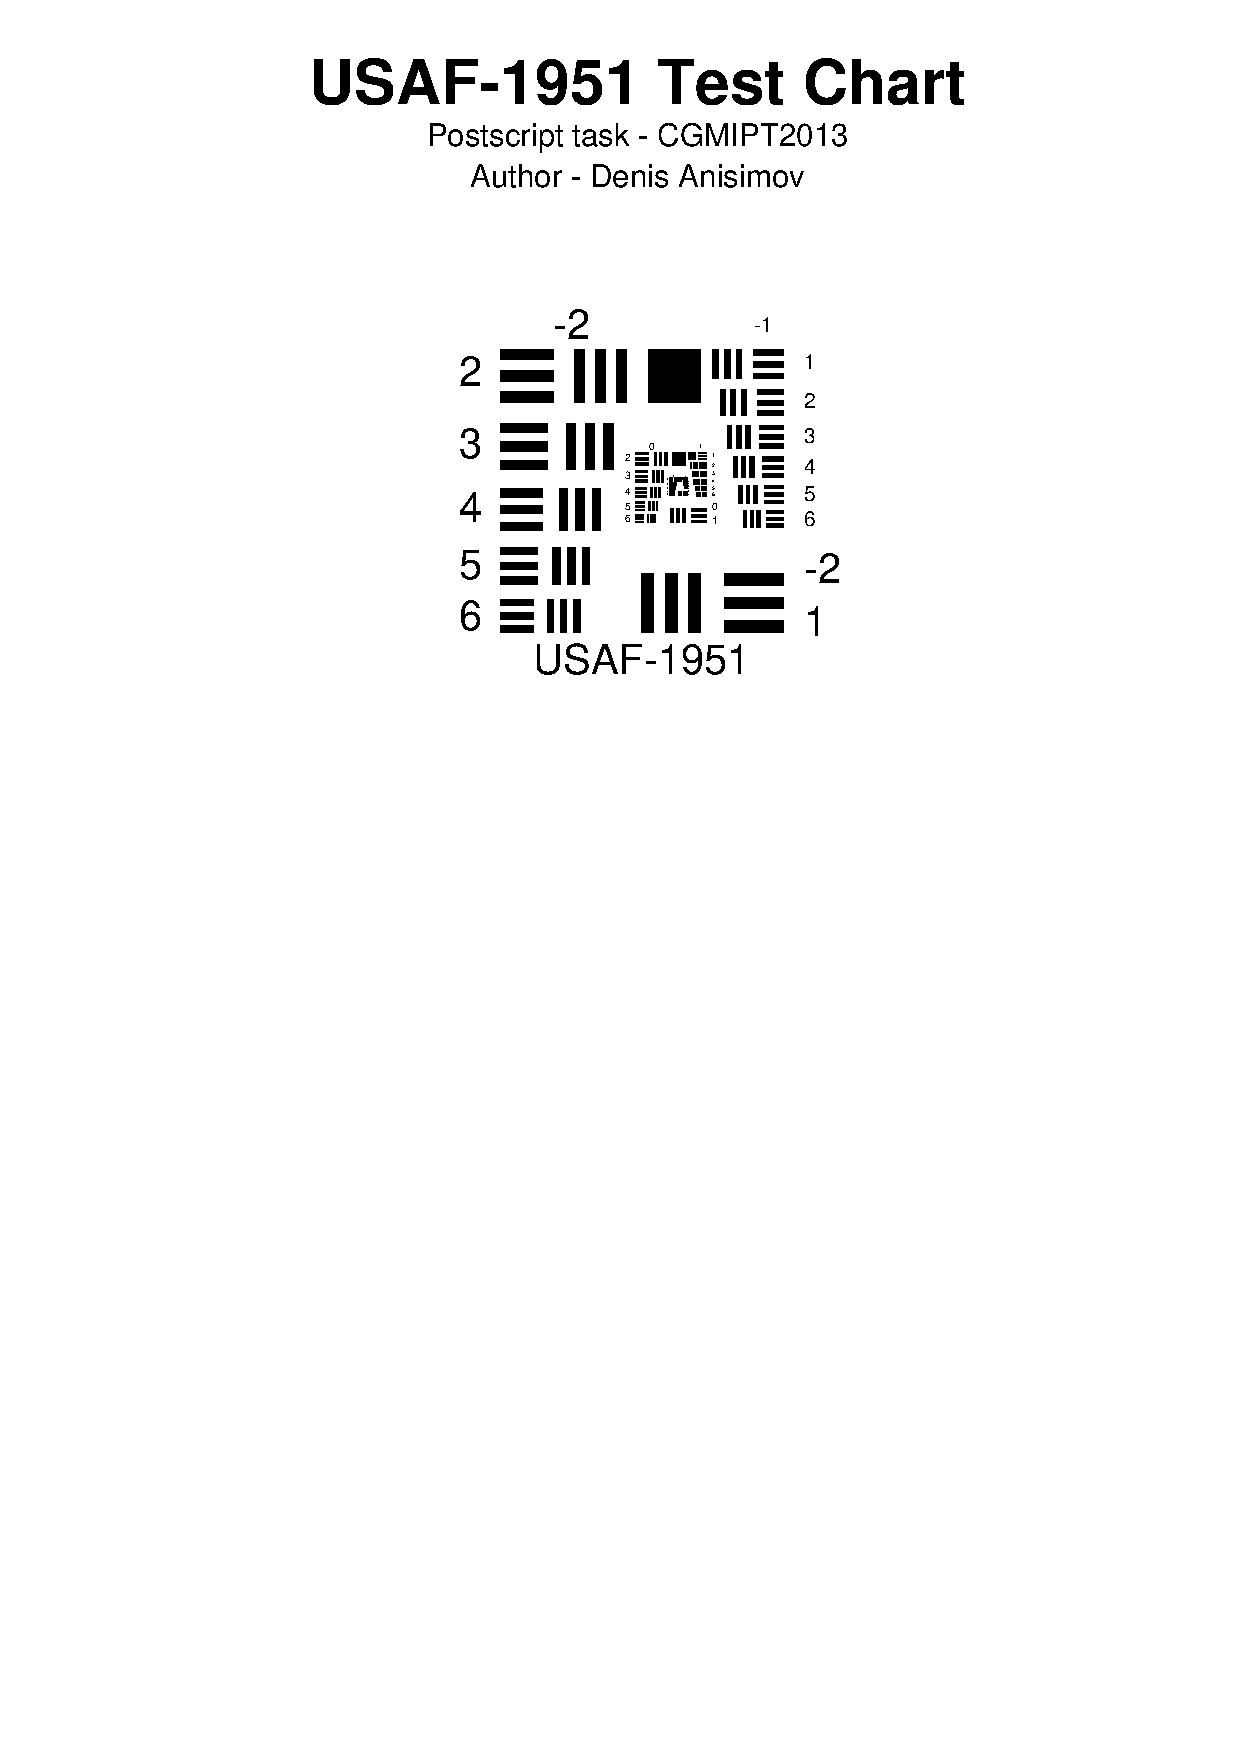
\includepdf{usaf1951.pdf}
\end{document}